\documentclass[journal]{IEEEtran}
\usepackage{graphicx}
\usepackage[scriptsize,labelformat=empty]{caption}
\renewcommand{\arraystretch}{1.1}

\begin{document}

% Don't change this portion-- it will format the section below for you.:)
\newcommand{\labtitlepage}{
	\onecolumn
	\thispagestyle{empty} \vspace*{\fill}
	\begin{center}
		\LARGE\labtitle \\ \bigskip \bigskip \large\name \\ \bigskip
		\labsection \\ \bigskip \labdate \\ \bigskip \bigskip
		\textbf{TA} \\ \taname \\ \bigskip \textbf{Lab Partners} \\
		\partnername \\
	\end{center}
	\vspace*{\fill} \vspace*{\fill} \newpage
	\setcounter{page}{1}
	\twocolumn
}

%% Change these variables
\newcommand{\labtitle}{Laboratory 1: Uncertainty And Statistics}
\newcommand{\name}{Vladimir Vysotsky}
\newcommand{\labsection}{Section 2, Wednesday 8AM}
\newcommand{\labdate}{January 21, 2015}
\newcommand{\taname}{Elwin Martin}
\newcommand{\partnername}{Francesco de Chirico}

%% This creates your lab cover page.
\labtitlepage

\section{Introduction}
Uncertainty is a fundamental fact of scientific measurements. No perfect
instruments exist, and to make proper use of imperfect measurements, the
imperfections must be quantified. Additionally, there must be mathematical
techniques for using the uncertainties in further calculations, in the form of
propogation of error.

This lab is designed to demonstrate a particular method of calculating the
uncertainty, in the form of the standard deviation, for ensembles of data of
various size, and how to then use these uncertainties in simple calculations.

In particular, for every ensemble, the measured average value (given N
measurements) is

\begin{equation}
\label{average}
\bar x = \frac{1}{N} \sum_{i=1}^N x_i
\end{equation}

The corresponding uncertainty can be represented as the standard deviation of
the ensemble.

\begin{equation}
\label{stdev}
\sigma _x = \sqrt{\frac{1}{N-1} \sum_{i=1}^N (x_i - \overline{x})^2}
\end{equation}

Knowing Equation ~\ref{average} and Equation ~\ref{stdev}, one can represent
all the relevant information of a measurement as 

\begin{equation}
\label{measurement}
x = \bar x \pm \sigma _{\bar x}
\end{equation}

These values can be used in further calculations, but the uncertainties must be
taken into account. If the calculation in question is a function of several
variables, for instance F = f(x, y), the uncertainty can be calculated using
the uncertainties of each of the variables as

\begin{equation}
\label{propogation}
\sigma _{\bar F} = \sqrt{ \left( \frac{\partial f}{\partial x} \right)^2 \left(
\sigma _{\bar x} \right)^2 + \left( \frac{\partial f}{\partial x} \right)^2
\left( \sigma _{\bar x}\right)^2}
\end{equation}

This identity can be extended to functions of multiple variables.

In this paper, these simple identities are used in the analysis of ensembles of
various sizes, and of the relationship in uncertainties between ensembles of
related data sets.

\section{Procedure and Setup}

The setup consists of a simple circuit that generates a voltaage with large,
random fluctuations using a Zener diode. Figure 2.1 illustrates the relevant
ports. 30 V DC will be the input, and $V_2$, $V_1$, and $V_{out}$ will all have
measurements taken from them - they will output a randomly fluctuating voltage.

First, measurements will only be taken on $V_1$, at varying ensemble sizes (but
always at 1,000 points per second). This will serve to demonstrate how standard
deviation changes as the ensemble size changes.

Then, measurements from both $V_1$ and $V_2$ will be taken, as well as the
measurement on $V_{out}$ after connecting $V_1$ and $V_2$ to $V_{in1}$ and
$V_{in2}$. These three ports implement a simple adding circuit, such that
$V_{out} = -(V_{in1} + V_{in2})$. This will allow a measurement to be taken
directly of the sum of $V_1$ and $V_2$, as well as adding together the
individual outputs of $V_1$ and $V_2$.

\begin{figure}[ht!]
\centering
\includegraphics[width=80mm]{circuit.png}
\caption{Figure 2.1: The relevant ports used in the circuit}
\end{figure}

Using Equation ~\ref{propogation}, and the fact that $V_{out} = -(V_1 + V_2)$,
the theoretical uncertainty of $V_{out}$ can be calculated using Equation
~\ref{voutunc}.

\begin{displaymath}
\sigma _{\bar V_{out}} = \sqrt{ \left( \frac{\partial (V_1 + V_2)}{\partial V_1}
\right)^2 \left( \sigma _{\bar V_1} \right)^2 + \left( \frac{\partial (V_1 +
V_2)}{\partial V_2} \right)^2 \left( \sigma _{\bar V_2}\right)^2}
\end{displaymath}

\begin{equation}
\label{voutunc}
\sigma _{\bar V_{out}} = \sqrt{ \left( \sigma _{\bar V_1} \right)^2 + \left(
\sigma _{\bar V_2}\right)^2}
\end{equation}

Though it is outside the scope of this setup, it is also worth deriving the
uncertainty for the current, given the voltage and resistance. It would be the
logical next step after verifying propogation of uncertainty in a voltage
adder.

Starting with the same propogation equation, for the function I = V/R, one gets.

\begin{displaymath}
\sigma _{\bar I} = \sqrt{ \left(\frac{1}{\bar R} \sigma _{\bar V} \right)^2 + 
\left( \frac{- \bar V}{\bar R^2} \sigma _{\bar R} \right)^2 }
\end{displaymath}

Squaring both sides, and factoring V/R out of the fractions

\begin{displaymath}
\left( \sigma _{\bar I} \right)^2 = \left( \frac{\bar V}{\bar R} \frac{\sigma
_{\bar V}}{\bar V} \right)^2 + \left( \frac{\bar V}{\bar R} \frac{\sigma _{\bar
R}}{\bar R} \right)^2
\end{displaymath}

Substituting I = V/R, and dividing both sides of the equation by it, one gets
the final identity.

\begin{equation}
\label{currentunc}
\left( \frac{\sigma _{\bar I}}{\bar I} \right)^2 = \left( \frac{\sigma _{\bar
V}}{\bar V} \right)^2 + \left( \frac{\sigma _{\bar R}}{\bar R} \right)^2
\end{equation}

\section{Data Analysis and Results}

Initially, measurements were taken only of $V_1$, a single random voltage
output.  Measurements were taken with ensemble sizes of 10, 100, 500, 1000,
5000, and 10000. For every data set size, ten individual ensembles were taken,
and the average and standard deviationn of each was recorded. The uncertainty
in each measurements was taken in one of two ways. Since the uncertainty is the
deviation of the mean, it could be taken directly from multiple ensembles by
taking the standard deviation of the means, using Equation ~\ref{stdev}. In
addition, the uncertainty of a single ensemble could be calculated using
Equation ~\ref{ensunc}.

\begin{equation}
\label{ensunc}
\sigma _{\bar V_{N}} = \frac{1}{sqrt{N}} \sigma _{N_{i}}
\end{equation}

These two values are presented in Graph 3.1 for every ensemble.

\begin{figure}[ht!]
\centering
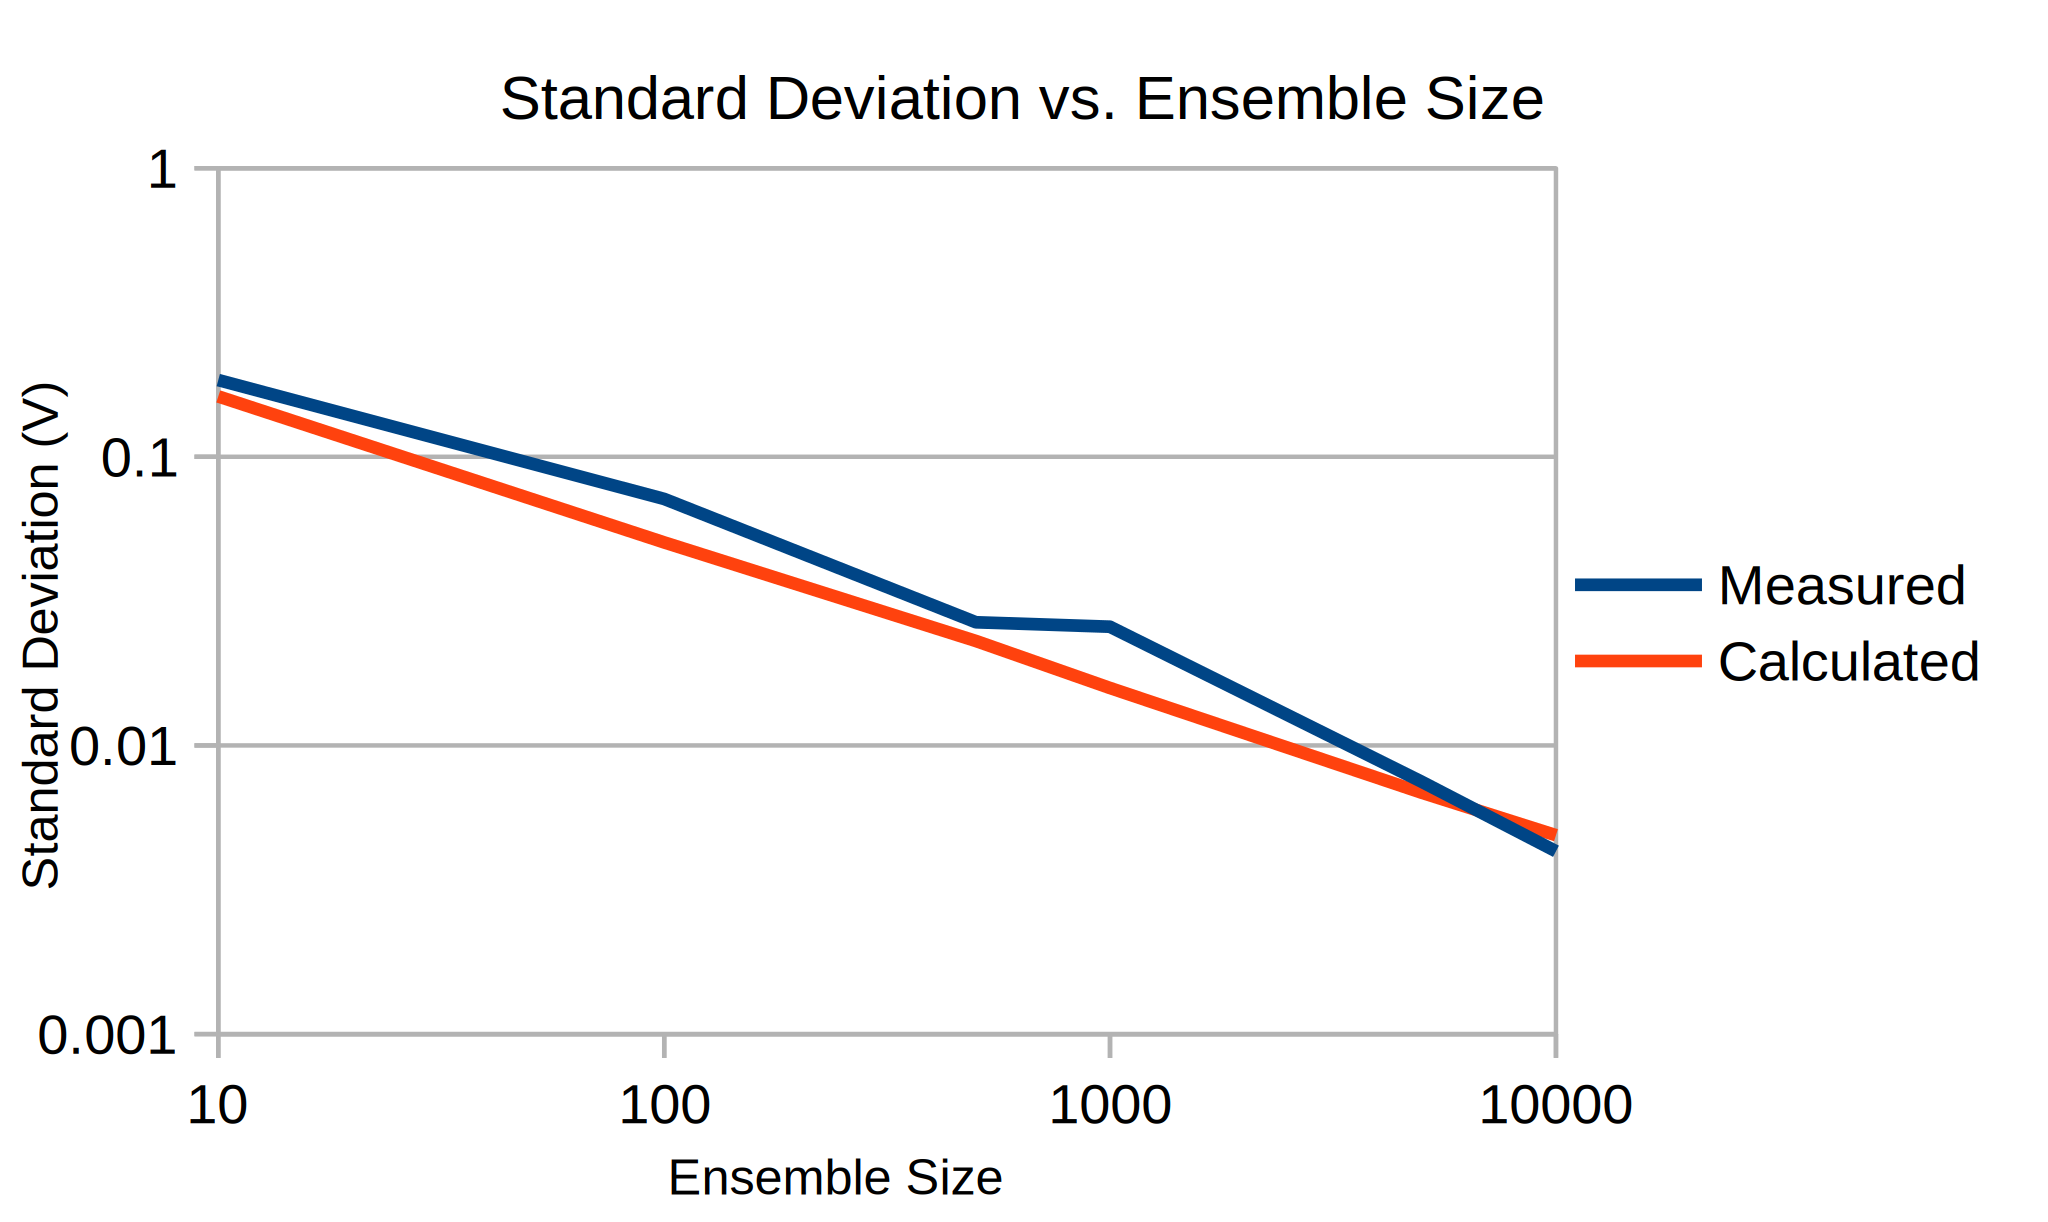
\includegraphics[width=80mm]{measure.png}
\caption{Graph 3.1 : Uncertainties in the measurements of randomly fluctuating
voltage, at varying ensemble sizes, on a log-log plot}
\end{figure}

The two methods of calculating uncertainty show good agreement, demonstrating
that the statistical method is in agreement with how uncertainty appears in
reality - that is, the statistical predictions of how much the average value
will vary at various ensemble sizes matches the real variation in average value
at the same ensemble size.

The voltage sources were then reconnected such that $V_1$ and $V_2$ could be
read independently, and were added together such that $-(V_1 + V_2)$ could be
read fromm $V_{out}$. In this case, there are two uncertainties that can be
calculated for $V_{out}$ - the statistical prediction from the individual
uncertainties of $V_1$ and $V_2$, and the real uncertainty calculated from
direct measurement of $V_{out}$ using Equation ~\ref{ensunc}.


\begin{table}[ht]
\centering
\caption{\normalsize{Voltage Measurements}}
\scalebox{.9}{
\begin{tabular}{|l|l|l|l|}
	\hline
	Input & Voltage (V) & $\sigma$ $_{V}$ (V) & $\sigma$ $_{\bar V}$ (V)      \\ \hline
	$V_1$ & -0.015 & 0.4856 & 0.0048         \\ \hline
	$V_2$ & 0.0044 & 0.5372 & 0.0054         \\ \hline
    $V_{out}$ & -0.002 & 0.6776 & 0.0068       \\ \hline
	\end{tabular}
}
\medskip
\caption{Table 3.1: Measurements of individual voltages and their sum in an
adder circuit.}
\end{table}

The real and predicted values for $V_{out}$'s uncertainty are presented in Table
3.2.

\begin{table}[ht]
\centering
\caption{\normalsize{Voltage Uncertainty Calculations}}
\scalebox{.9}{
\begin{tabular}{|l|l|l|}
	\hline
	& $V_{out}$ (V) &  $\sigma _{\bar V_{out}}$ (V)      \\ \hline
	Measured & -0.002 & 0.0068         \\ \hline
	Calculated & -0.0053 & 0.0072      \\ \hline
	\end{tabular}
}
\medskip
\caption{Table 3.2: Measured and calculated uncertainties for the summed
voltage.}
\end{table}

The values of $V_{out}$ match to within the uncertainty, but more important, the
uncertainties themselves are very similar. Error propogation appears to match
the reality of how random fluctuations propogate in a physical system, in this
case overestimating slightly (which is alright in terms of uncertainty, as long
as the measurement is still usable).

The other common case for uncertainty propogation is a product of several
uncertain values. This case does not arise naturally in the measurement of
voltages, but since the statistical methods worked so far, it would be
reasonable to surmise they would also work for products. With this motivation,
the following is a quick derivation of the uncertainty for a function f(x, y) =
xy, using Equation ~\ref{propogation}.

\begin{displaymath}
\sigma _{\bar f} = \sqrt{ \left( \frac{\partial}{\partial x} xy  \right)^2
\left( \sigma _{\bar x} \right)^2 + \left( \frac{\partial}{\partial y} xy
\right)^2 \left( \sigma _{\bar y} \right)^2 }
\end{displaymath}

\begin{equation}
\label{product_unc}
\sigma _{\bar f} = \sqrt{ \left( y \sigma _{\bar x} \right)^2 + \left( x
\sigma_{\bar y} \right)^2 }
\end{equation}

It is useful to get a qualitative feel for how the uncertainty of the product
changes with the uncertainties and relative sizes of the two inputs. Table 3.3
summarizes this when $\bar x = \bar y = 1$.

\begin{table}[ht]
\centering
\caption{\normalsize{Relative Uncertainty Propogation}}
\scalebox{.9}{
\begin{tabular}{|l|l|l|}
	\hline
	$\sigma _{\bar x}$ & $\sigma _{\bar y}$ &  $\sigma _{\bar f}$ (V)      \\ \hline
	0.1 & 0.1 & 0.14         \\ \hline
	0.1 & 0.01 & 0.1005      \\ \hline
	0.1 & 0.001 & 0.1000      \\ \hline
	0.1 & 0 & 0.1      \\ \hline
	\end{tabular}
}
\medskip
\caption{Table 3.3: Uncertainty propogation when relative input uncertainty
decreases.}
\end{table}

The uncertainty of the product depends heavily on the relative uncertainties of
each term, to the point where when one is ten times smaller the result is
negligible, and when it's 100 times smaller it is not distinguishable from 0.

\section{Conclusion}

The observation of the voltage adder system supports the statistical prediction
about how uncertainty is propogated, at least for simple arithmetic operations.
If a system physically adds two quantities, the resulting data will exhibit
uncertainty according to Equation ~\ref{propogation}.

This has not been verified for products, in particular the prediction of
Equation ~\ref{product_unc}, or for more complex functions. Some functions
could be tested with the current setup - for instance, Equation
~\ref{currentunc} could be tested by measuring either the current or resistance
in the circuit and calculating the other. More complex functions would require
extra testing.


\ifCLASSOPTIONcaptionsoff
  \newpage
\fi

\end{document}


